\documentclass{article}
\usepackage{graphicx} % Required for inserting images
\usepackage[T2A]{fontenc}
\usepackage{tikz}
\thispagestyle{empty}
%\usetikzlibrary{positioning}

\begin{document}
{\small Для вдумчивого читателя заметим, что \hspace{5pt}
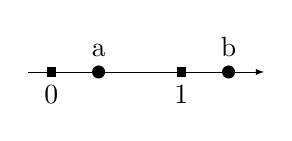
\begin{tikzpicture}
    \draw[black, line width=0.05pt, -latex] (0,0) -- (3,0)
    node[pos=0.1,scale=0.5, fill=black,label=below:\textcolor{black}{0}]{}
    node[pos=0.3,scale=0.5, shape=circle, fill=black,label=above:\textcolor{black}{a}]{}
    node[pos=0.65,scale=0.5, fill=black,label=below:\textcolor{black}{1}]{}
    node[pos=0.85,scale=0.5, shape=circle, fill=black,text=green,label=above:\textcolor{black}{b}]{};
\end{tikzpicture} \\
ссылка в начале параграфа на то, что дей- \\
ствительные числа и их свойства известны  \\
из курса элементарной математики, не яв- \hspace{30pt} Рис. 3 \\
ляется необходимой. Сформулированные \\
выше свойства действительных чисел можно взять за исход- \\
ное определение. Следует только исключить тривиальный слу- \\
чай: легко проверить, что для множества, состоящего только \\
из одного нуля, выполняются все свойства I—V (в таком мно- \\
жестве 0 = 1). Множество, в котором имеется хоть один эле- \\
мент, отличный от нуля, будем здесь для краткости называть \\
нетривиальным. \par
Перефразируя сказанное, получим следующее определе- \\
ние. \\
\
\textbf{Определение 1.} \textit{Нетривиальное множество элементов, об- \\
ладающих свойствами I—V, называется множеством дей- \\
ствительных чисел. Каждый элемент этого множества \\
называется действительным числом.} \par
Построение теории действительных чисел, основывающее- \\
ся на таком их определении, называется \textit{аксиоматическим}, \\
а свойства I—V — \textit{аксиомами действительных чисел}. \par
Геометрически множество действительных чисел изобра- \\
жается направленной (ориентированной) прямой, а отдель- \\
ные числа — точками этой прямой. Поэтому совокупность \\
действительных чисел часто называют числовой прямой, а \\
также числовой или действительной осью, а отдельные чис- \\
ла — ее точками (рис. 3). \par
При такой интерпретации действительных чисел иногда \\
вместо a меньше b (a больше b) говорят, что точка a лежит \\
левее точки b (что a лежит правее b). \par
В п. 2.2*—2.6° будут более детально проанализированы \\
свойства I-V действительных чисел и выведены некоторые \\
их следствия. Как и все пункты, отмеченные звездочками, \\
эти пункты при первом чтении можно без существенного \\
ущерба для усвоения курса математического анализа опус- \\
тить. Для понимания дальнейшего материала (в § 3 и следую- \\
щих) вполне достаточно представления о действительных \\
числах, которое дается в курсе элементарной математики. \\
\section*{\textbf{2.2*. Свойства сложения и умножения}}
Рассмотрим некоторые свойства сложения и умножения, ко- \\
торые вытекают из свойств I, II и III. Прежде всего заметим, \\
\centerline{
\begin{tikzpicture}
    \draw (0,0) -- (1.5,0);
\end{tikzpicture} 
}
\\
\centerline{\textit{39}}
}
\end{document}
